\documentclass[UTF8,a4paper]{ctexart}
\usepackage{graphicx}
\usepackage{geometry}
\geometry{a4paper,scale=0.8}
\usepackage{setspace}
\setstretch{1.6}

\begin{document}
\begin{sloppypar}
	
	\begin{center}
		\begin{fontsize}{80pt}{20pt}
			实验报告
		\end{fontsize}

		\bigskip
		\bigskip
		
		\begin{fontsize}{35pt}{20pt}
			\begin{flushright}
				———用{\Huge Shell}工具和脚本与{\Huge Vim}编辑器来进行数据整理
			\end{flushright}
		\end{fontsize}
		
		\bigskip
		\bigskip
		\bigskip
		\bigskip
		\bigskip
		\bigskip
		\bigskip
		\bigskip
		\bigskip
		\bigskip
		\bigskip
		\bigskip
		\bigskip
		\bigskip
		\bigskip
		\bigskip
		\bigskip
		\bigskip
		\bigskip
		\bigskip
		\bigskip
		\bigskip
		
		\begin{fontsize}{25pt}{20pt}
			姓名:
			\underline{翟一航}
			
			\bigskip
			\bigskip
			\bigskip
			\bigskip
			
			学号:
			\underline{{\huge 23020011046}}
			
			\bigskip
			\bigskip
			\bigskip
			\bigskip
			
			班级:
			\underline{{\Huge 23}级软件工程五八班}
			
			
		\end{fontsize}
	\end{center}
	\section{实验要求}
	\subsection{学会使用Shell工具来进行脚本编写和运行}
	\subsection{学会利用Vim编辑器来进行更高效的文本编辑和数据整理}
	\subsection{完成至少4个课堂练习与20个与Shell和Vim有关的实例}
	\section{实验内容}
	\subsection{Shell的学习}
	\subsubsection{Shell 是一个命令行界面和脚本语言,用于与操作系统交互。它充当用户和系统之间的接口,解释和执行命令,并允许编写脚本以自动化任务。常见的Shell包括Bash、sh、zsh、csh 和ksh,它们各自提供不同的功能和特性,以满足各种用户需求。}
	\subsubsection{Shell主要具有以下功能:\\1.命令解释器:Shell 解释并执行用户输入的命令。这些命令可以是系统内置的,也可以是外部程序或脚本。\\2.脚本语言:Shell 提供了一种编程环境,允许用户编写脚本来自动化各种任务,如文件操作、系统管理、批处理等。\\3.用户界面:Shell 可以提供命令行界面(CLI),通过它,用户可以直接输入命令和参数来控制计算机系统。}
	\subsubsection{常见的Shell类型包括:\\1.Bash:这是最常用的 Linux 和macOS的默认Shell,兼容BourneShell(sh),并加入了许多增强特性。在本次实验中,我主要使用Git(bush)来进行Shell指令和运用的学习。\\2.sh:这是最早的Unix Shell,由Steve Bourne开发。\\3.zsh:提供了比Bash更强大的功能和更多的扩展,通常用于高级用户和开发者。\\4.csh :它的语法与 C 语言类似,主要用于一些特定的 Unix 系统。\\5.ksh:由 David Korn 开发,融合了 sh 和 csh 的特性,并提供了额外的功能。}
	\subsection{Vim编辑器的学习}
	\subsubsection{Vim是一款高度可定制的文本编辑器,基于早期的 Vi 编辑器,提供了许多增强功能。它主要用于编写和编辑源代码,但也可以用于一般的文本编辑。}
	\subsubsection{Vim拥有如下特点:\\1.模式编辑:Vim 采用模式化编辑方式,主要有三种模式:普通模式(用于导航和操作文本)、插入模式(用于输入文本)和命令模式(用于执行命令)。这种模式化设计使得编辑过程更高效。\\2.强大的快捷键和命令:Vim 提供了丰富的快捷键和命令,支持复杂的文本操作和导航,提高编辑效率。\\3.可定制性:用户可以通过配置文件(如 .vimrc)定制 Vim 的行为和外观,安装插件以扩展其功能。\\4.跨平台:Vim 支持多种操作系统,包括 Unix/Linux、macOS 和 Windows,使得它在不同平台上的使用都很便利。}
	\subsection{使用Vim和awk进行数据整理}
	\subsubsection{使用awk进行数据整理}
	awk是一个强大的文本处理工具,特别擅长处理结构化文本数据,如 CSV 文件。它通过模式匹配和操作字段来进行数据提取和处理。基本用法包括选择字段、字段分隔符、条件筛选、数据处理等。
	\subsubsection{使用Vim进行数据整理}
	Vim是一个强大的文本编辑器,适合于手动编辑和处理文本数据。通过搜索与替换、模式匹配和删除、分割和合并文件、宏录制、列操作等功能可以进行数据整理。
	\subsubsection{结合使用awk和Viim}
	在将二者结合使用的过程中,一般先使用awk处理和提取数据,生成初步整理的结果文件,再在Vim中进一步编辑与格式化数据,以满足特定需求或进行复杂的手动调整。Vim与awk的结合使用,可以使得数据整理工作更加高效和精准。
	\subsection{课堂练习}
	\graphicspath{{figure/}}
	\subsubsection{阅读 man ls ,然后使用 ls 命令进行如下操作:
		\\1. 所有文件(包括隐藏文件)
		\\2. 文件打印以人类可以理解的格式输出 (例如,使用 454M 而不是 454279954)
		\\3. 文件以最近访问顺序排序
		\\4. 以彩色文本显示输出结果}
	
	\bigskip
	\bigskip
	\bigskip
	\bigskip
	
	打开Git(Bush),在初始位置即可进行该课堂练习的操作。尝试后发现,在Git(Bush)中并没有man这一功能,也没有fd这一功能,不过存在find功能,在此就不在查看ls的具体功能,直接开始课堂练习。
	
	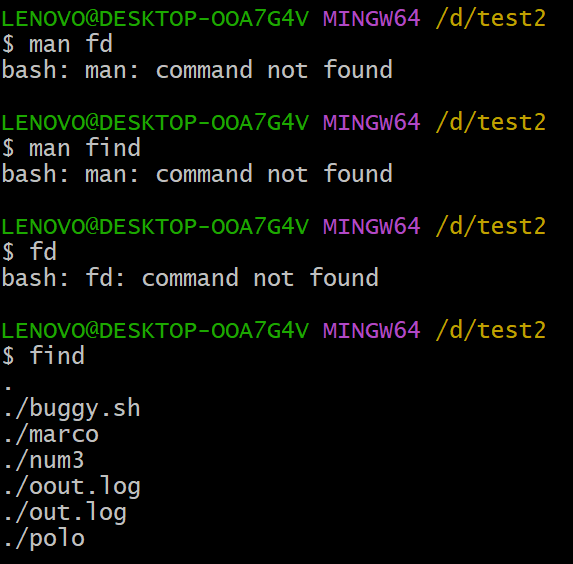
\includegraphics[width = 12cm]{0}
	
	1.如果要查看所有的文件,包括隐藏文件,我们可以使用命令ls -a(或者ls -l,不过该命令为显示所有文件以及其详细信息),结果如下:
		
	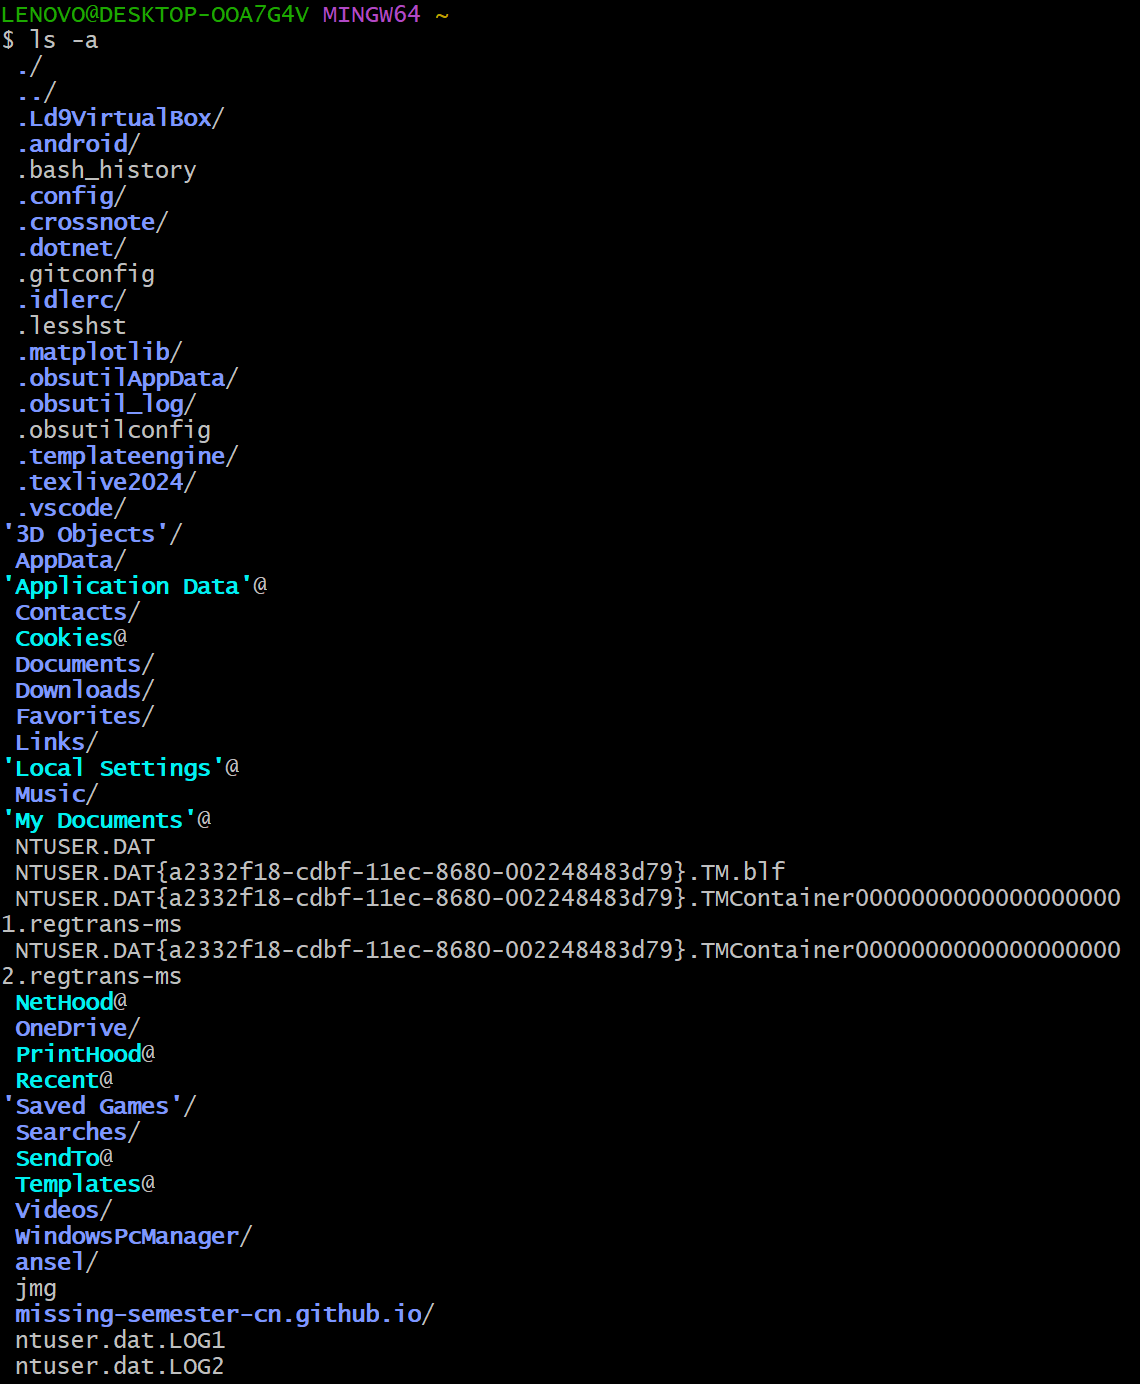
\includegraphics[width = 16cm]{1}

	(该图片为ls -a的结果)

	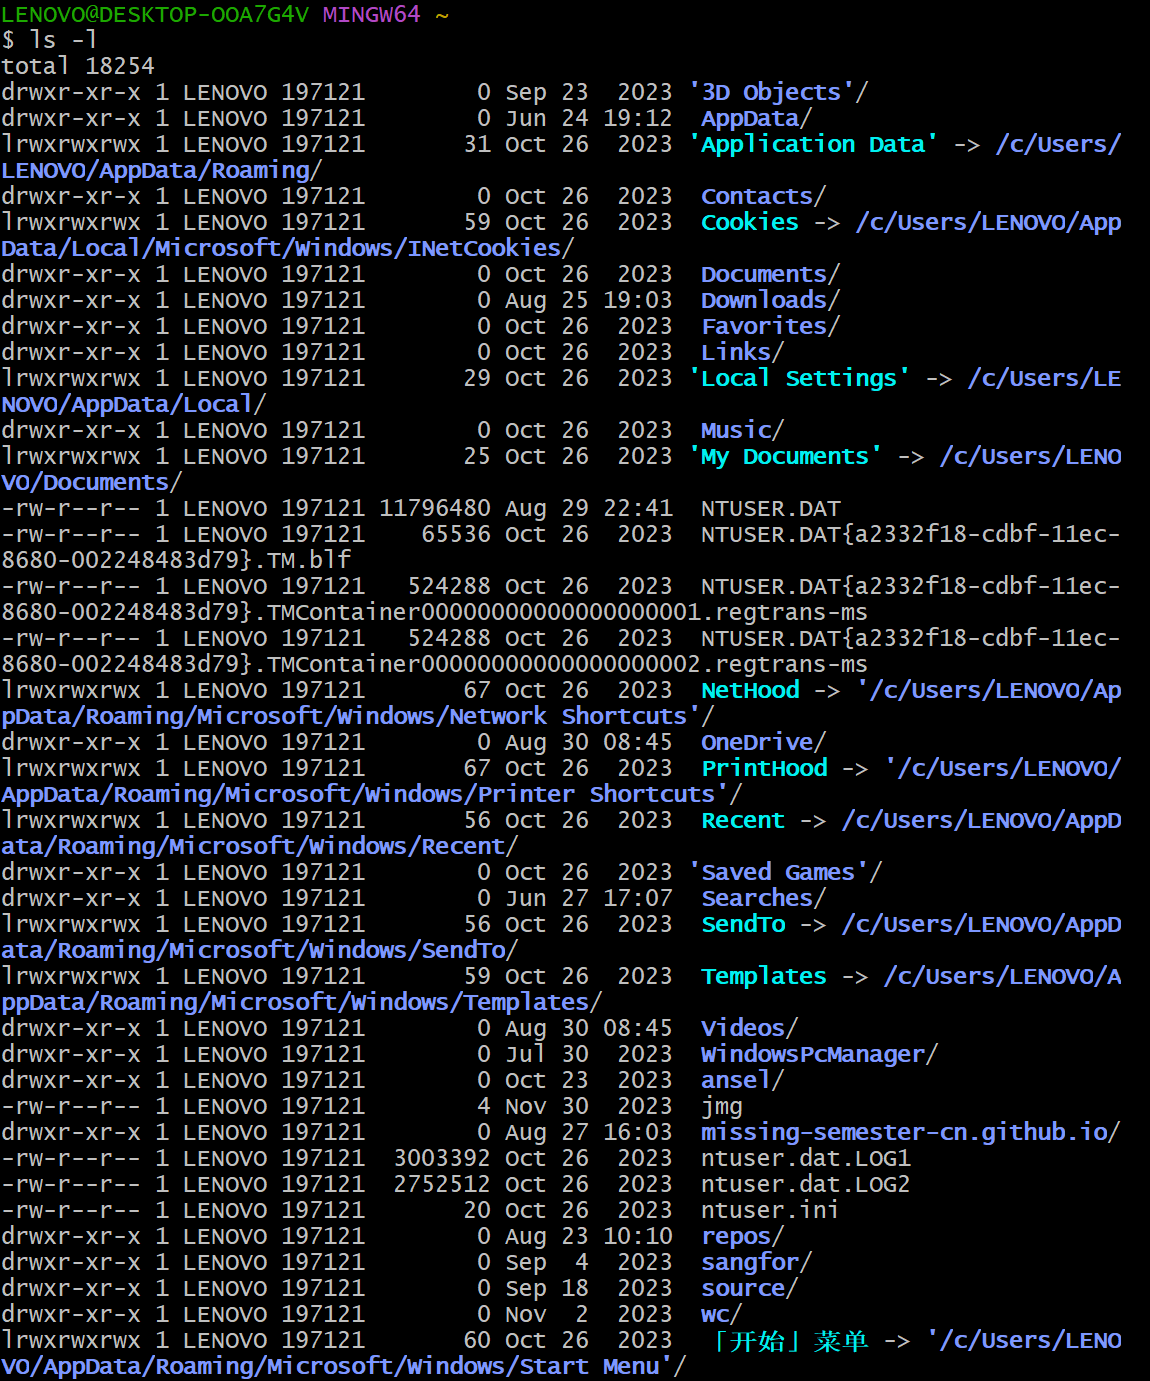
\includegraphics[width = 16cm]{2}
	
	(该图片为ls -l的结果,可以看出所展示的信息要更为详细)

	2.显示文件,并将文件打印以人类可以理解的格式输出,在此我们需要输入指令ls -h。结果如下图。
	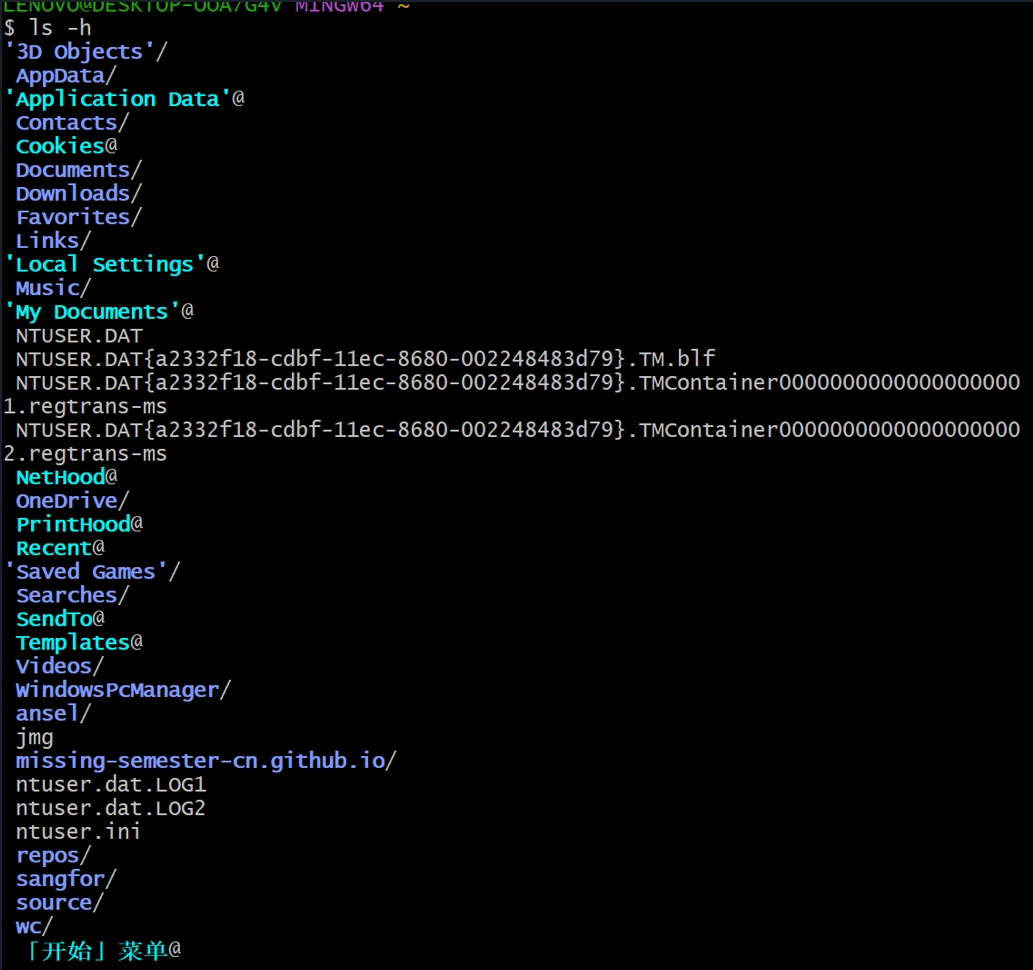
\includegraphics[width = 16cm]{3}

	3.将文件以最近访问顺序排序,用到指令ls -h。结果如下图。
	
	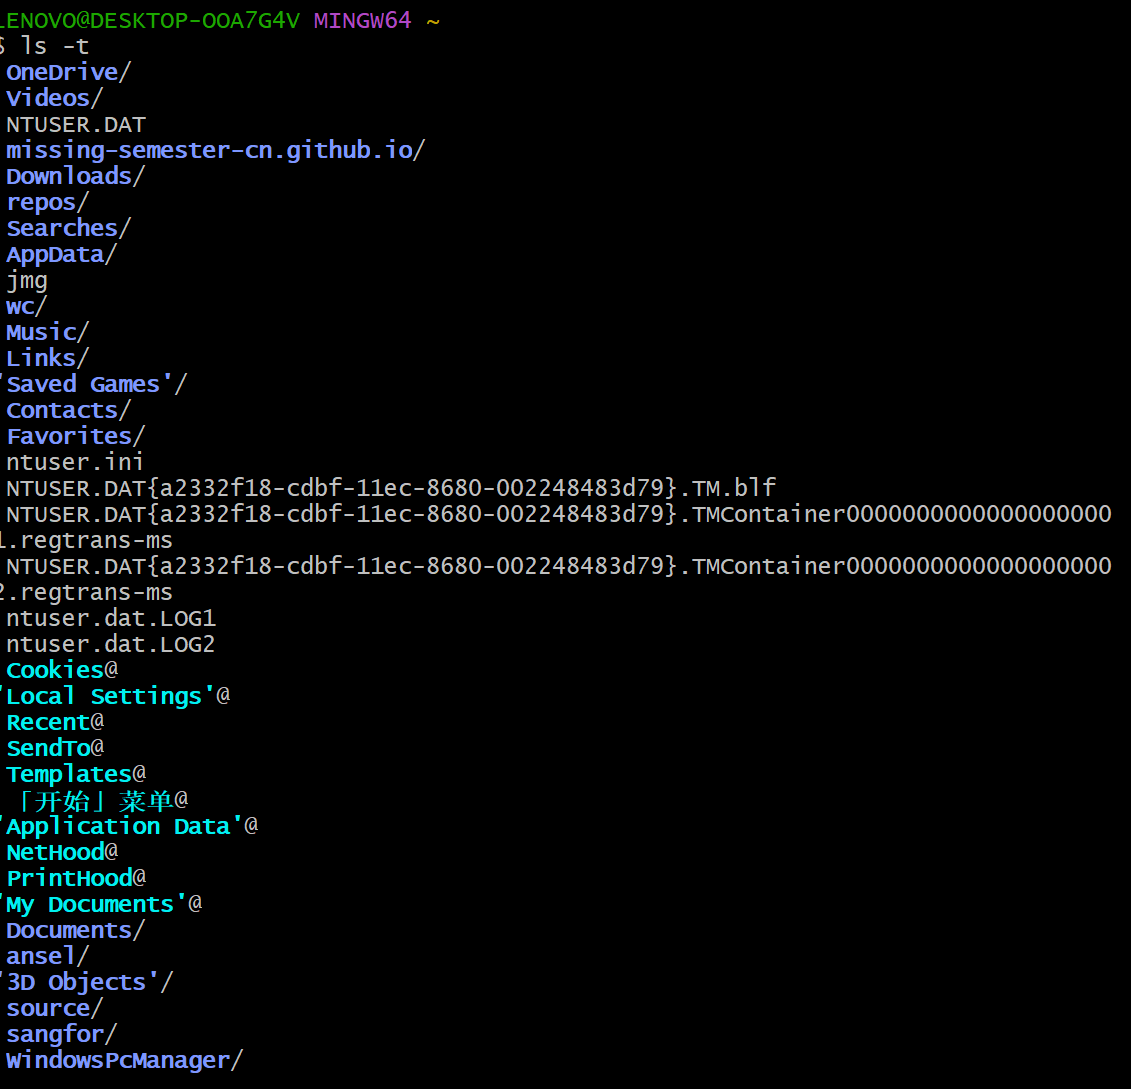
\includegraphics[width = 16cm]{4}

	4.以彩色文本显示输出结果,正常情况下需要输入指令ls --color=auto,不过由于使用的Git(Bush)自带了该功能,故与上述结果有些相似。结果如图。
	
	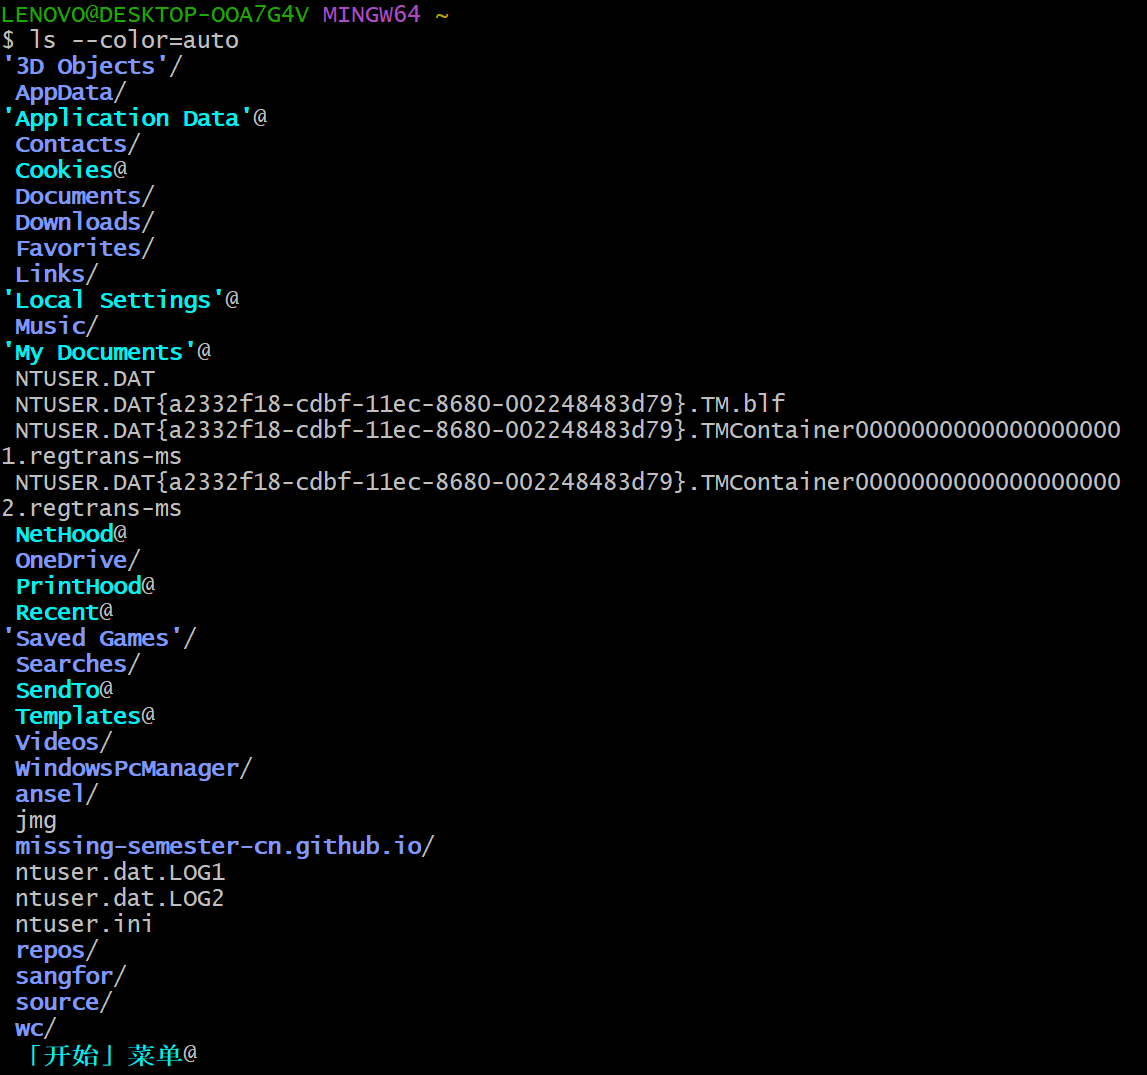
\includegraphics[width = 16cm]{5}
	
	\subsubsection{编写两个 bash 函数 marco 和 polo 执行下面的操作。 每当你执行 marco 时,当前的工作目录应当以某种形式保存,当执行 polo 时,无论现在处在什么目录下,都应当 cd 回到当时执行 marco 的目录}
	在此处我首先通过vim编辑功能,创建了两个脚本文件marco和polo,用来写入需要的代码,如图
	

	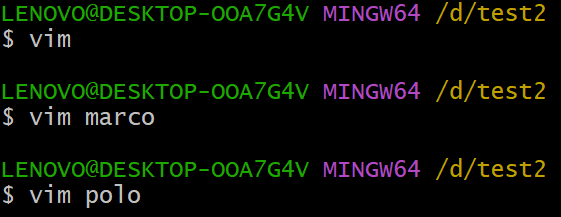
\includegraphics[width = 16cm]{6}

	然后开始编写marco和polo这两个函数,函数内容如下图所示:

	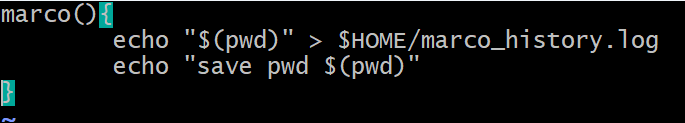
\includegraphics[width = 16cm]{7}

	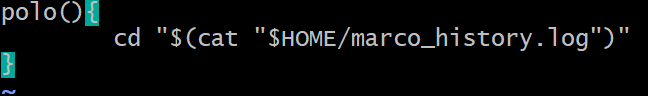
\includegraphics[width = 16cm]{8}
	
	\subsubsection{假设您有一个命令,它很少出错。因此为了在出错时能够对其进行调试,需要花费大量的时间重现错误并捕获输出。 编写一段 bash 脚本,运行如下的脚本直到它出错,将它的标准输出和标准错误流记录到文件,并在最后输出所有内容。 加分项:报告脚本在失败前共运行了多少次。}

	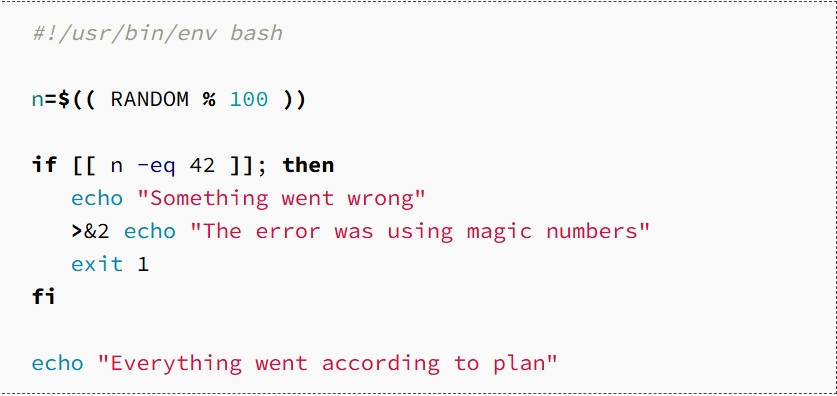
\includegraphics[width = 16cm]{9}
	
	首先,创建一个文件名为buggy.sh用来存放上述脚本,然后,创建一个num3脚本用来运行buggy.sh。 num3的具体内容如下:

	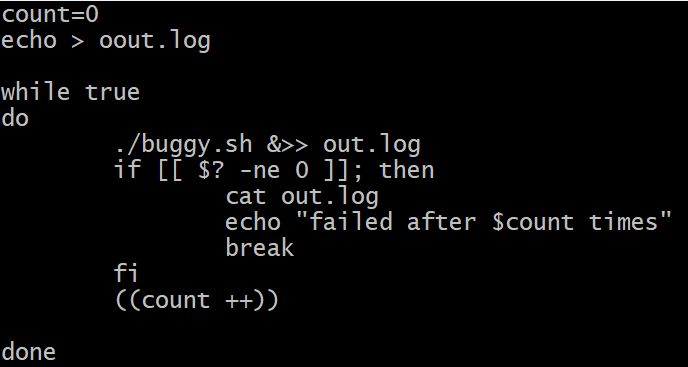
\includegraphics[width = 12cm]{10}

	运行结果为:

	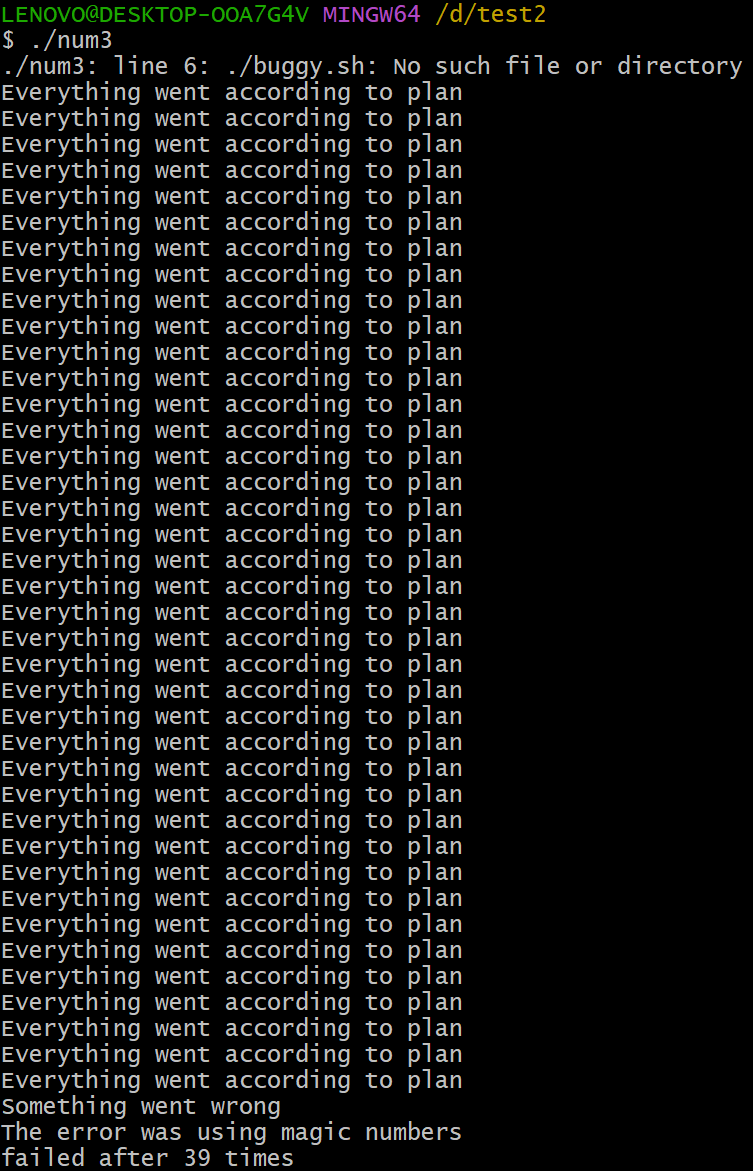
\includegraphics[width = 10cm]{11}

	由此可知,该buggy.sh脚本在运行39次后出现错误。

	\subsubsection{编写一个命令,它可以递归地查找文件夹中所有的 HTML 文件,并将它们压缩成 zip 文件。注意,即使文件名中包含空格,您的命令也应该能够正确执行}
	
	首先我们使用mkdir创建所需要的文件夹,然后再执行find命令find html\_root -name "*.html" -print0 | xargs -0 tar vcf html.zip,即可查找文件夹中所有的HTML文件,并将它们压缩为zip文件。

	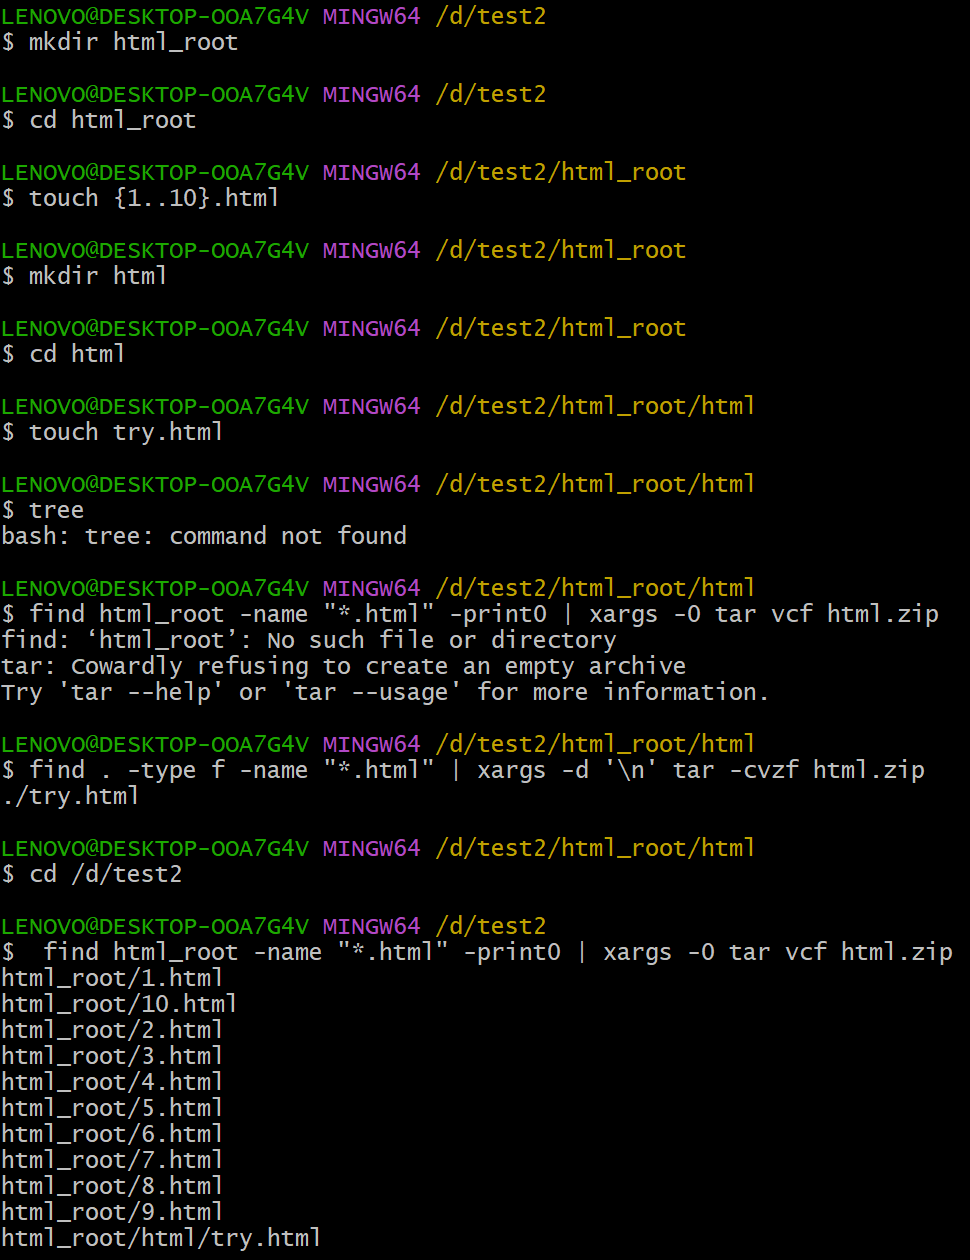
\includegraphics[width = 16cm]{12}

	
	\subsubsection{编写一个命令或脚本递归的查找文件夹中最近使用的文件。}
	输入指令find . -type f -print0 | xargs -0 ls -lt | head -1即可完成该任务。
	
	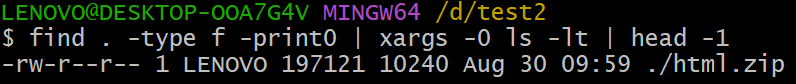
\includegraphics[width = 16cm]{13}
	
	\section{实验中遇到的问题与解决方法}
	\subsection{想用man指令查看相关语句含义时,出现该指令无效的提示}

	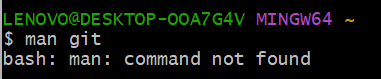
\includegraphics[width = 16cm]{14}

	要想解决这个问题,首先用which命令检查man命令的安装情况,显示no man in……则表明没有安装man命令,此时输入命令sudo apt-get install man-db,将man命令安装并放到相应的路径中,即可使用man命令查看相关命令的功能。
	\subsection{在进行课堂练习4创建文件并对文件做出相关操作时,执行find命令时显示无法找到相关文件}
	
	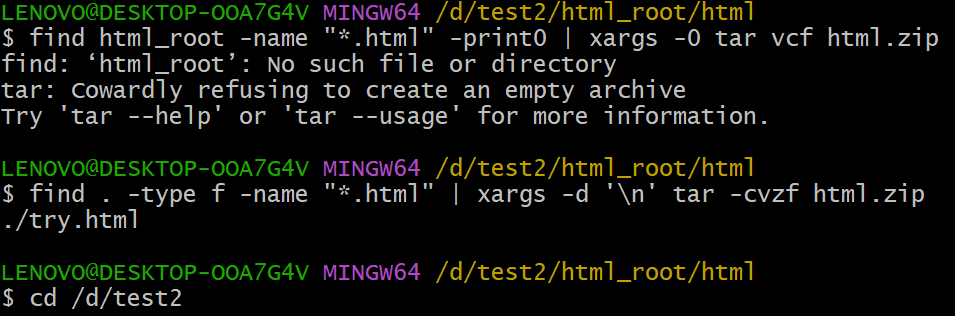
\includegraphics[width = 16cm]{15}

	这是因为创建文件后在文件夹的最小html文件中,不是在文件夹的目录中,因而find命令找不到具体执行的目标,应该返回到文件夹所在目录,在进行find操作。
	
	\section{实例练习}
	\subsection{查看当前所在路径}
	输入命令pwd,即可查看当前所在路径。

	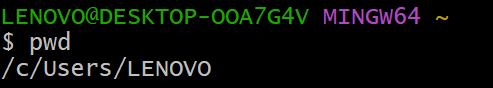
\includegraphics[width = 12cm]{16}
	
	\subsection{创建脚本文件}
	输入命令touch 文件名即可创建脚本文件。

	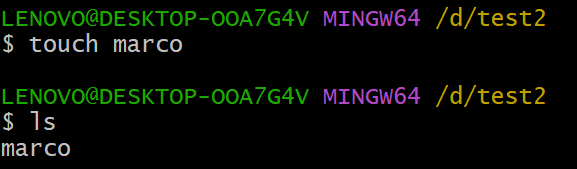
\includegraphics[width = 12cm]{17}

	\subsection{运行脚本文件}
	./文件名,即可运行。

	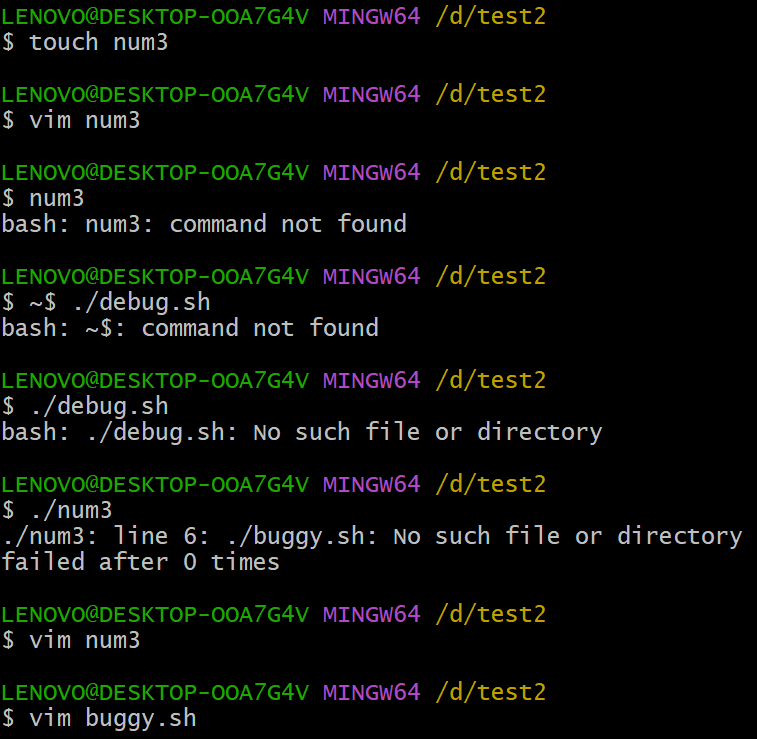
\includegraphics[width = 12cm]{18}
	
	\subsection{打印}
	创建脚本文件,并进入编辑模式,利用echo语句即可打印相关的内容
	
	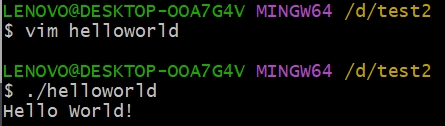
\includegraphics[width = 12cm]{19}
	
	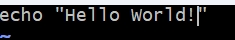
\includegraphics[width = 12cm]{20}
	
	\subsection{统计当前目录下的文件数目}
	编写脚本(如图),然后运行即可
	
	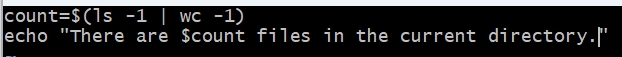
\includegraphics[width = 12cm]{21}
	
	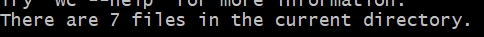
\includegraphics[width = 12cm]{22}
	
	\subsection{按时间戳备份文件}
	编写脚本(如图),然后运行即可
	
	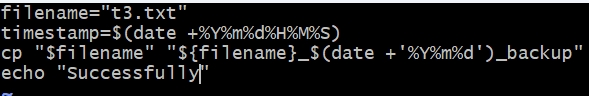
\includegraphics[width = 12cm]{23}
	
	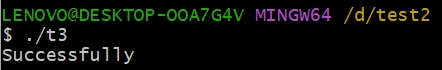
\includegraphics[width = 12cm]{24}
	
	\subsection{在当前目录及其子目录中删除空的子目录。}
	首先在当前目录中创建空文件夹t4,然后编写脚本并运行(如图)
	
	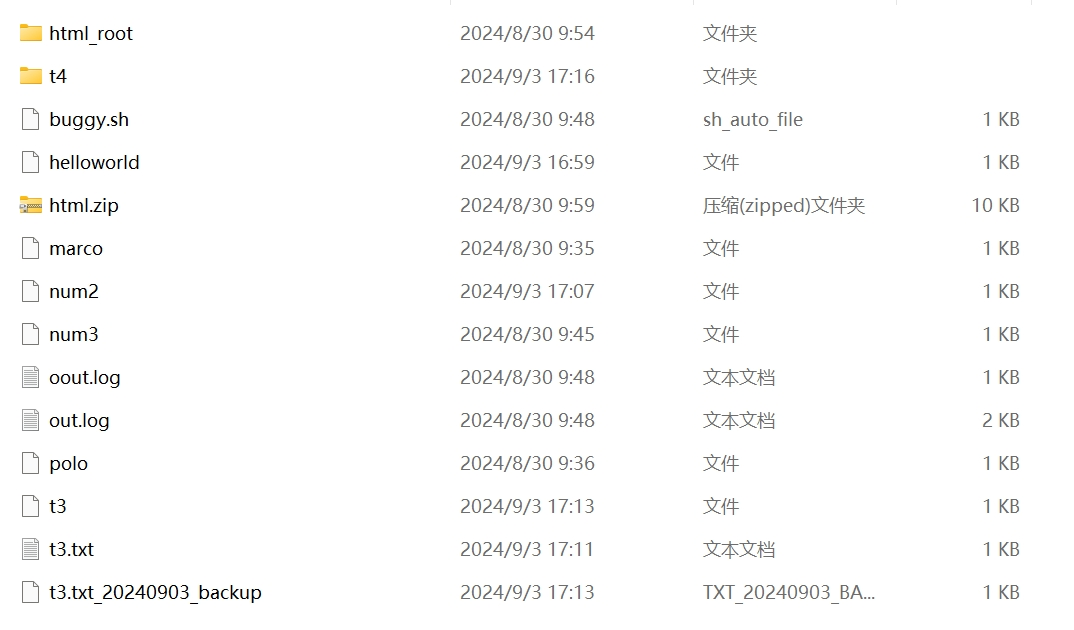
\includegraphics[width = 12cm]{25}
	
	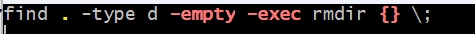
\includegraphics[width = 12cm]{26}
	
	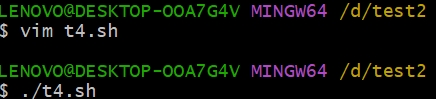
\includegraphics[width = 12cm]{27}
	
	删除后的目录如图所示,可见删除成功
	
	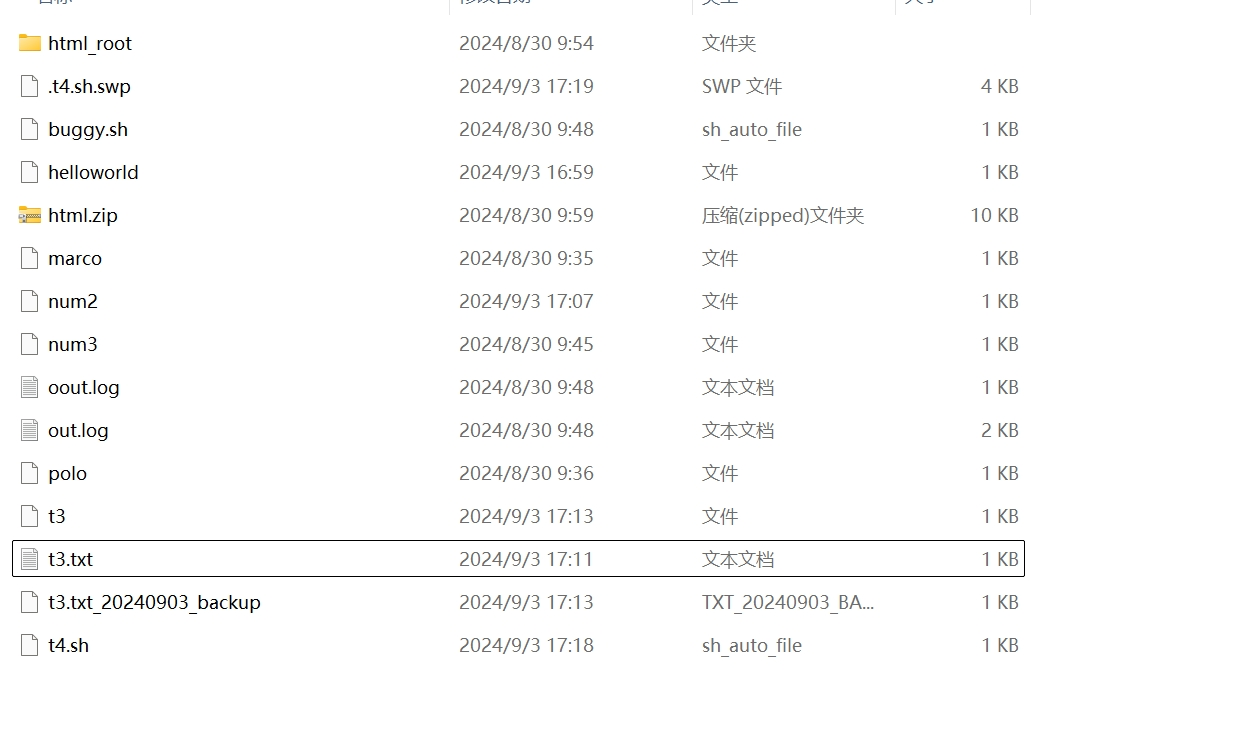
\includegraphics[width = 16cm]{28}
	
	\subsection{进程监控与重启}
	编写脚本如下
	
	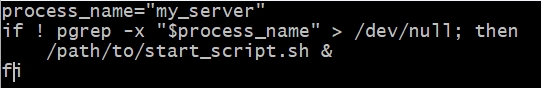
\includegraphics[width = 13cm]{29}
	
	\subsection{定时执行任务}
	创建一个每分钟执行的任务,并执行。
	
	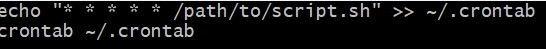
\includegraphics[width = 12cm]{30}
	
	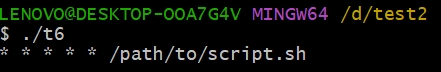
\includegraphics[width = 12cm]{31}
	
	\subsection{文件内容替换}
	替换文本文件中的特定字符串:用 new\_string 替换 old\_string,并将结果保存到 t7.txt 中。
	
	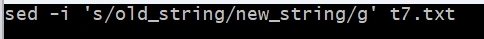
\includegraphics[width = 12cm]{32}
	
	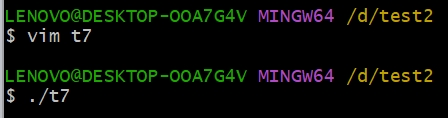
\includegraphics[width = 12cm]{33}
	
	文件t7.txt前后变化如图:
	
	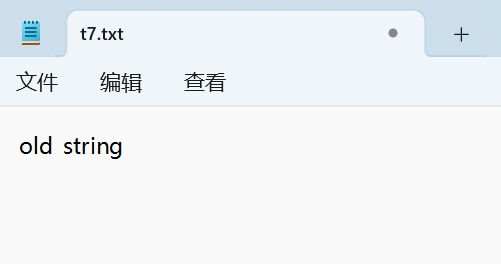
\includegraphics[width = 8cm]{34}
	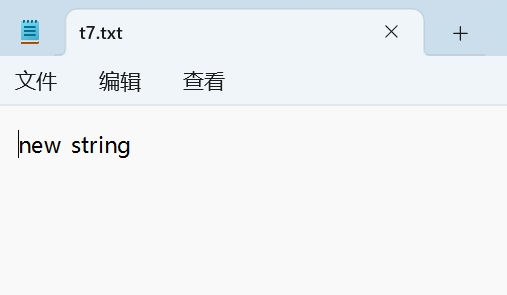
\includegraphics[width = 8cm]{35}
	
	\subsection{批量重命名文件}
	将目录中的txt文件全部修改为md文件。
	
	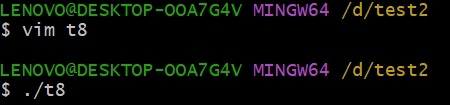
\includegraphics[width = 12cm]{360}
	
	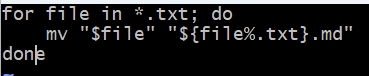
\includegraphics[width = 12cm]{36}
	
	脚本运行前后txt文件变化:
	
	
\includegraphics[width = 16cm]{37}
	
	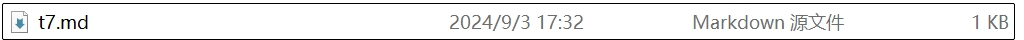
\includegraphics[width = 16cm]{38}
	
	\subsection{查找并删除指定名称的文件}
	查找并删除当前目录及其子目录下指定名称的文件。此处删除t7.md文件为例,由于结果显著且简单,此处不再展示图片。
	
	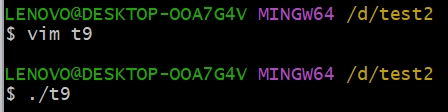
\includegraphics[width = 12cm]{39}
	
	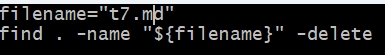
\includegraphics[width = 12cm]{40}
	
	\subsection{检查网络连接}
	测试网络连通性
	
	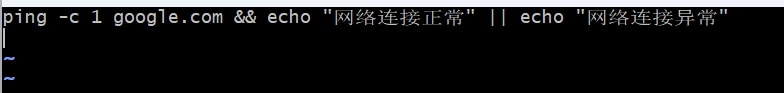
\includegraphics[width = 12cm]{41}
	
	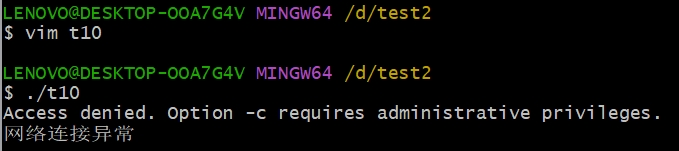
\includegraphics[width = 12cm]{42}
	
	\subsection{打开并保存文件}
	打开文件:vim filename.txt
	
	保存文件::w 或 :wq(保存并退出)
	
	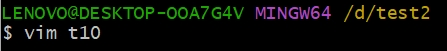
\includegraphics[width = 12cm]{43}
	
	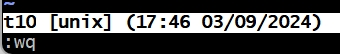
\includegraphics[width = 12cm]{44}
	
	\subsection{文本编辑}
	
	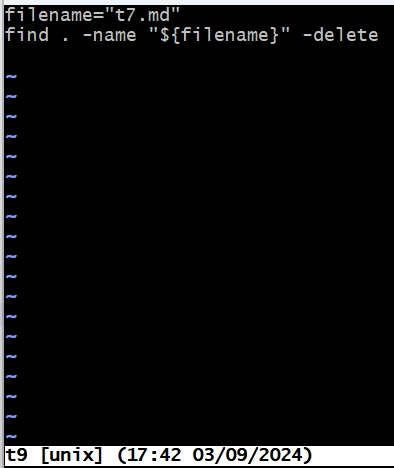
\includegraphics[width = 8cm]{45}
	
	i:在当前光标处进入插入模式
	
	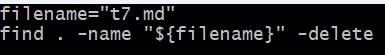
\includegraphics[width = 10cm]{46}
	
	a:在当前光标的下一个字符位置进入插入模式
	
	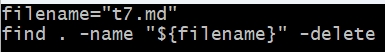
\includegraphics[width = 10cm]{47}
	
	o:在当前行下方插入新行并进入插入模式
	
	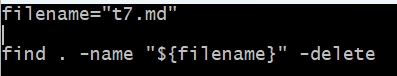
\includegraphics[width = 10cm]{48}
	
	\subsection{移动光标}
	
	\includegraphics[width = 8cm]{49}
	
	w:移动到下一个单词的开头
	
	\includegraphics[width = 10cm]{50}
	
	b:移动到前一个单词的开头
	
	\includegraphics[width = 10cm]{51}
	
	gg:跳转到文件的第一行
	
	\includegraphics[width = 10cm]{52}
	
	G:跳转到文件的最后一行
	
	\includegraphics[width = 10cm]{53}
	
	\subsection{复制和粘贴}
	yy:复制当前行
	P(大写):粘贴到光标后
	
	\includegraphics[width = 10cm]{55}
	
	p(小写):粘贴到光标前
	
	\includegraphics[width = 10cm]{54}
	
	\subsection{设置行号}
	:set number或者简写为:set nu
	
	\includegraphics[width = 8cm]{56}
	
	\subsection{分割窗口}
	水平分割窗口::split 或简写为 :sp
	
	\includegraphics[width = 16cm]{57}
	
	垂直分割窗口::vsplit 或简写为 :vsp
	
	\includegraphics[width = 16cm]{58}
	
	在新窗口中打开文件::sp filename.txt(new.txt为新创建的空文件)
	
	\includegraphics[width = 16cm]{59}
	
	\subsection{多文件编辑}
	使用vim打开多个文件:vim file1.txt file2.txt
	
	\includegraphics[width = 16cm]{60}
	
	在文件间切换::next(:n)到下一个文件,:prev(:p)到上一个文件
	
	\includegraphics[width = 8cm]{61}
	\includegraphics[width = 8cm]{62}

	列出所有打开的文件::buffers
	
	\includegraphics[width = 12cm]{63}
	
	\section{实验收获与感悟}
	学习Shell脚本与工具让我深刻体会到自动化操作的力量,它们极大地提高了处理系统任务和批量文件操作的效率。尽管Shell脚本的灵活性和可移植性带来便利,但也需注意不同Linux环境间的差异。与高级语言相比,Shell脚本更侧重于系统级任务的快速实现,展现了其独特的价值。
	
	Vim编辑器以其高效和灵活著称,通过掌握其多种模式和快捷键,我能够显著提升文本编辑的速度和效率。然而,Vim的学习曲线较为陡峭,需要时间和实践来适应其独特的操作方式。尽管如此,一旦掌握,Vim的强大功能和扩展性将为我提供无尽的便利和可能性。
	
	将Vim和awk结合使用进行数据整理,我感受到了两者在文本处理方面的强大互补性。Vim提供了便捷的文本编辑功能,而awk则擅长复杂的数据分析和处理。这种协同工作的方式不仅提高了数据整理的效率和准确性,还让我在实践中不断发现新的应用场景和解决方案,进一步加深了对这两个工具的理解和掌握。
	
	Github仓库链接:https://github.com/Locusclaer/-.git
	
\end{sloppypar}
\end{document}